\documentclass[../main.tex]{subfiles}
\graphicspath{{figures/}{../figures/}}

\begin{document}

\noindent\textbf{Step 1 分析调头区域}
\par 根据题目要求,舞龙队在调头空间内的运动轨迹大致如下:
\begin{figure}[H]
\centering
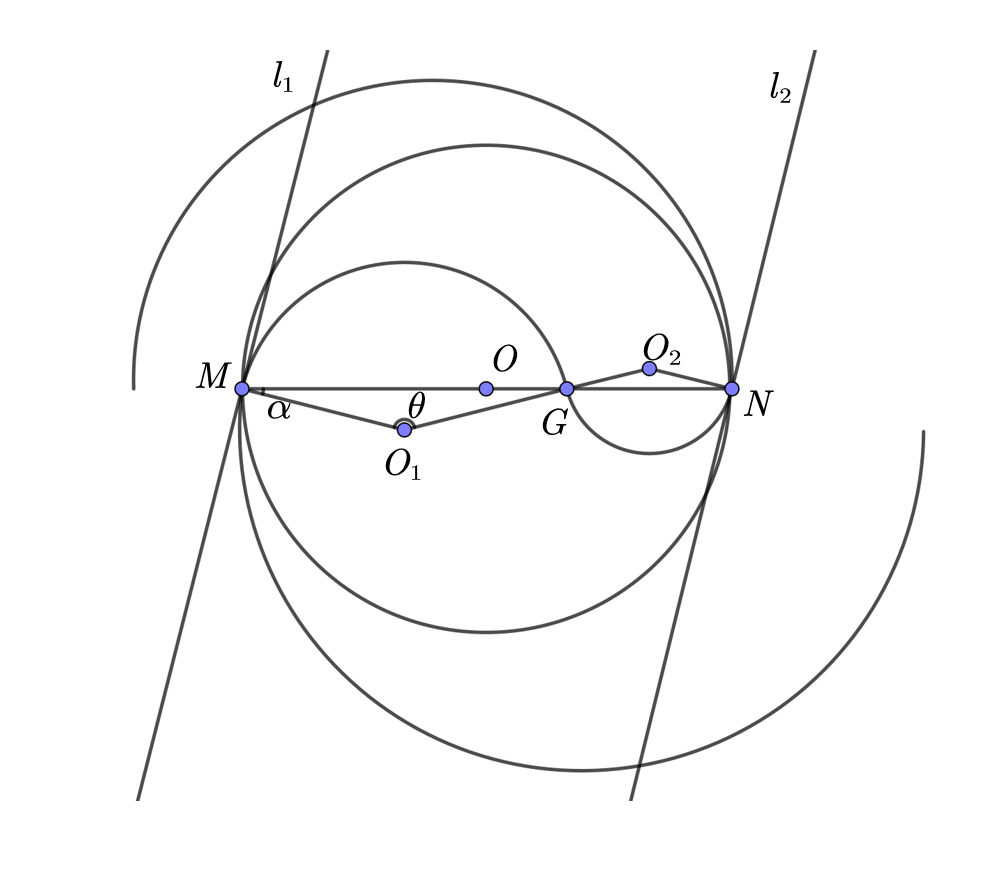
\includegraphics[width=.6\textwidth]{4}
\caption{调头空间示意图}
\label{2.2.2.2.2.2} 
\end{figure}
\par 其中,盘入螺线与盘出螺线与调头区域边界交点分别为$M$和$N$。前一段、后一段调头圆弧圆心分别为$O_1$,$O_2$.两段圆弧切点为$G$.过点$M$与盘入螺线相切的直线为$l_M$,过点$N$与盘出螺线相切的直线为$l_N$。记第一段圆弧半径与调头空间直径的夹角为$\alpha $,第一段圆弧对应的夹角为$\theta $。
\\ 根据题目和计算可以得到以下结论:
\begin{itemize}
\item  由于两段圆弧之间相切,所以$O_1,G,O_2$三点共线。
\item  经计算可知,$\angle MGO_2+\angle O_2GN=\pi $,基于这个条件,可得M,G,N三点共线。
\item  因为盘入螺线$\varGamma$与盘出螺线$\varGamma'$中心对称,所以$MN$一定过原点$O$且$l_M$平行于$ l_N$。
\item  由于两段圆弧均与盘入,盘出螺线相切,因此$O_1M\bot l_M${,}$O_2N\bot l_N$且$O_1M$与$O_2N$的大小比例为2:1。
\item  由于$O_1M $平行于$ O_2N$,则由几何关系易得
\begin{gather}
\angle MO_1G=\angle NO_2G=\theta,\label{1.........33}
\\
\angle O_1MN=\angle O_1GMN=\angle O_2GN=\angle O_2NG=\alpha .\label{1.........34}
\end{gather}
\end{itemize} 
\noindent\textbf{Step 2 证明不可通过改变前后两段调头圆弧半径比例减小调头曲线长度} 
\par 记调头区域半径为$R$,则$\left| \overrightarrow{OM} \right|=\left| \overrightarrow{ON} \right|=R$. 设前后两段调头圆弧半径比例为$a:1$,记后一段调头圆弧的半径为$r$,则前一段调头圆弧的半径为$ar$,其中$a$为任意常数.则
\begin{align}\label{1.........35}
\left| \overrightarrow{O_1M} \right|=\left| \overrightarrow{O_1G} \right|=ar,\left| \overrightarrow{O_2N} \right|=\left| \overrightarrow{O_2G} \right|=r.    
\end{align}
\par 设直线$l_M,$ $l_N,$ $O_1M,$ $MN$的斜率分别为$k_{l_M},$ $k_{l_N},$ $k_{O_1M},$ $k_{MN}$,根据两直线夹角斜率公式可得
\begin{align}\label{1.........36}
\tan \alpha =\tan \angle NMO_1=\frac{k_{MN}-k_{l_{O_1M}}}{1+k_{MN}k_{l_{O_1M}}}.
\end{align}
\par 从而
\begin{align}\label{1.........37}
\alpha =\left| \arctan \frac{k_{MN}-k_{l_{O_1M}}}{1+k_{MN}k_{l_{O_1M}}} \right|.
\end{align}
\par 由\(O_1M\parallel O_2N\),\(\angle MO_1G=\angle NO_2G\) ,\(\angle O_1MG=\angle O_2NG\) ,且\(\vert\overrightarrow{O_1M}\vert = 2\vert\overrightarrow{O_2N}\vert\) ,根据角角边定理可得$\vartriangle MO_1G\cong \vartriangle NO_2G$,由此可得下述线段比例关系
\begin{align}\label{1.........38}
\left| \overrightarrow{NG} \right|=\frac{\left| \overrightarrow{MN} \right|}{1+a}=\frac{2R}{1+a}.
\end{align}
\par 再结合几何关系易得
\begin{align}\label{1.........39}
\theta =\pi -2\alpha ,\quad \cos \alpha =\frac{\frac{1}{2}\left| \overrightarrow{NG} \right|}{\left| \overrightarrow{O_2N} \right|}=\frac{R}{\left( 1+a \right) r}.
\end{align}
\par 因此
\begin{align}\label{1.........40}
r=\frac{R}{\left( 1+a \right) \cos \alpha}.
\end{align}
\par 设$\wideparen{MG}$的长度为$L_1$,$\wideparen{GN}$的长度为$L_2$,记$L=L_1+L_2$.于是根据圆弧长度计算公式可得
\begin{align}\label{equation-1}
L=L_1+L_2=\theta r+\theta ar=\left( 1+a \right) \theta r=\frac{\left( \pi -2\alpha \right) R}{\cos \alpha}=\frac{\left( \pi -2\left| \arctan \frac{k_{MN}-k_{l_{O_1M}}}{1+k_{MN}k_{l_{O_1M}}} \right| \right) R}{\cos \left| \arctan \frac{k_{MN}-k_{l_{O_1M}}}{1+k_{MN}k_{l_{O_1M}}} \right|}.
\end{align}
\par 由上式可知$L$与$a$无关,因此不可通过改变前后两段调头圆弧半径比例减小调头曲线长度.

\noindent\textbf{Step 3 调头曲线长度} 
\par 由Step 2可知调头曲线长度与$MN$以及盘入螺线在M处的斜率$k_{l_{O_1M}}$有关,因此我们需要确定$M$,$N$的位置,记它们的极坐标分别为$(\rho_M,\theta_M)$和$(\rho_N,\theta_N)$。由图2可知,$M$与$N$分别为盘入螺线,盘出螺线与调头空间的交点。
\par 其中, 盘入螺线\(\varGamma\)的极坐标方程和直角坐标方程分别为
\begin{gather}
\varGamma :\rho =\frac{d_0}{2\pi}\theta.\label{7.3.1}
\\
\varGamma :\begin{cases}\label{7.4.1}
x=\frac{d_0}{2\pi}\theta \cos \theta\\
y=\frac{d_0}{2\pi}\theta \sin \theta\\
\end{cases}
\end{gather}

\par 由于盘入螺线与盘出螺线关于螺线中心呈中心对称,因此盘出螺线$\varGamma'$的极坐标方程和直角坐标方程分别为
\begin{gather}
\varGamma':\rho =\frac{d_0}{2\pi}\left( -\theta \right) .\label{7.3.2}  \\
\varGamma':\begin{cases}\label{7.4.2}
x=\frac{d_0}{2\pi}\left( -\theta \right) \cos \theta\\
y=\frac{d_0}{2\pi}\left( -\theta \right) \sin \theta\\
\end{cases}
\end{gather}

\par 由于调头空间的直径为R,因此其极坐标方程为
\begin{align}
S:\rho =R. \label{7.3.3} 
\end{align}
\par 因此,将\eqref{7.3.3}式分别与\eqref{7.3.1}式,\eqref{7.3.2}式联立得到$M$,$N$的极坐标
\begin{gather}\label{1.........41}
\begin{cases}
\rho _M=R\\
\theta _M=\frac{2\pi R}{d_0}\\
\end{cases}
\quad,
\begin{cases}
\rho _N=R\\
\theta _N=-\frac{2\pi R}{d_0}\\
\end{cases}.
\end{gather}
\par 通过坐标转化方程,将M,N的极坐标转化为直角坐标
\begin{gather}\label{1.........42}
\begin{cases}
x_M = R\cos\frac{2\pi R}{d_0}\\
y_M = R\sin\frac{2\pi R}{d_0}\\
\end{cases}
\quad,
\begin{cases}
x_N = R\cos(\frac{2\pi R}{d_0}-\pi)= - R\cos\frac{2\pi R}{d_0}\\
y_N = R\sin(\frac{2\pi R}{d_0}-\pi)= - R\sin\frac{2\pi R}{d_0}
    \\
\end{cases}.
\end{gather}
\par 于是得到MN的斜率
\begin{align}
k_{MN}=\tan\frac{2\pi R}{d_0}.\label{7.3.4}
\end{align}
\par 将\eqref{7.4.1}分别对x和y对于$\theta $求导
\[
\begin{cases}\label{1.........44}
\frac{dx}{d\theta} = \frac{d_0}{2\pi} (\cos\theta - \theta\sin\theta) \\
\frac{dy}{d\theta} = \frac{d_0}{2\pi} (\sin\theta + \theta\cos\theta)
\end{cases}
\]
\par 于是就有
\begin{align}\label{1.........45}
    \text{k}_{l_M}=\frac{\text{d}y}{dx}\mid _{M}^{}=\frac{\text{d}y/\text{d}\theta}{dx/\text{d}\theta}\mid _{M}^{}=\frac{\sin \theta +\theta \cos \theta}{\cos \theta -\theta \sin \theta}\mid _{\theta =\theta _M}^{}=\frac{\sin \frac{2\pi R}{d_0}+\frac{2\pi R}{d_0}\cos \frac{2\pi R}{d_0}}{\cos \frac{2\pi R}{d_0}-\frac{2\pi R}{d_0}\sin \frac{2\pi R}{d_0}}
\end{align}
\par 所以将\eqref{7.3.4} \eqref{1.........45}代入可得
\begin{align}\label{1.........46}
L =
\end{align}
\noindent\textbf{Step 4 计算圆心和切点的坐标}     
\begin{enumerate}
\item \textbf{切点坐标}
\end{enumerate} 
\par 通过题目给定条件,我们可以知道,前一段圆弧的半径是后一段的2倍,又由于$\vartriangle MO_1G\cong \vartriangle NO_2G$,所以$\vec{MG}=2\vec{GN}$,记G的直角坐标为$(x_{G},y_{G})$
\begin{gather}\label{1.........47}
\overrightarrow{MG}=\left( x_G-x_M,y_G-y_M \right) ,
\\
\overrightarrow{GN}=\left( x_N-x_G,y_N-y_G \right) .
\end{gather}
\par 在Step 3中我们已经求出M,N的直角坐标,因此
\begin{align}\label{1.........48}
\begin{cases}
x_G= -\frac{1}{3}R\cos\frac{2\pi R}{d_0}\\
y_G=-\frac{1}{3}R\sin\frac{2\pi R}{d_0}\\
\end{cases}.
\end{align}
\begin{enumerate}[start=2]
\item \textbf{圆心坐标}
\end{enumerate}   
\par 设前一段调头圆弧圆心$O_1$的直角坐标与极坐标分别为$(x_{O_1},y_{O_1})$和$(\rho_{O_1},\theta_{O_1})$,后一段调头圆弧圆心$O_2$的直角坐标为$(x_{O_2},y_{O_2})$和$(\rho_{O_2},\theta_{O_2})$.前一段圆弧的半径为$2r$,后一段圆弧的半径为r,因为圆心到圆上任意一点的距离相同,因此
\begin{gather}\label{1.........49}
|\overrightarrow{O_1O_2}|= |\overrightarrow{O_1G}| + |\overrightarrow{O_2G}| = 3r\\
|\overrightarrow{O_1M}|=2r   \\
|\overrightarrow{O_2M}|=r
\end{gather}
\par 即
\begin{gather}
2R=\left| \overrightarrow{MN} \right|=\left| \overrightarrow{MG} \right|+\left| \overrightarrow{GN} \right|= 2r\cos\alpha\times2 + r\cos\alpha\times2 = 6r\cos\alpha,
\\
\begin{cases}\label{1.........50}
\left( x_M-x_{O_1} \right) ^2+\left( y_M-y_{O_1} \right) ^2=4r^2\\
\left( x_G-x_{O_1} \right) ^2+\left( y_G-y_{O_1} \right) ^2=4r^2\\
\end{cases},
\\
\begin{cases}\label{1.........51}
\left( x_N-x_{O_2} \right) ^2+\left( y_N-y_{O_2} \right) ^2=r^2\\
\left( x_G-x_{O_2} \right) ^2+\left( y_G-y_{O_2} \right) ^2=r^2\\
\end{cases}.
\end{gather}
\par 由上式解得
\begin{gather}\label{1.........52}
\begin{cases}
x_{O_1}=\\
y_{O_1}=\\
\end{cases},\quad \begin{cases}
x_{O_2}=\\
y_{O_2}=\\
\end{cases}.
\end{gather}
\par  进而得到
\begin{gather}\label{1.........53}
\begin{cases}
\rho _{O_1}=\sqrt{x_{O_1}^{2}+y_{O_1}^{2}}=\\
\theta _{O_1}=\arctan \frac{y_{O_1}}{x_{O_1}}=\\
\end{cases},\quad \begin{cases}
\rho _{O_2}=\sqrt{x_{O_2}^{2}+y_{O_2}^{2}}=\\
\theta _{O_2}=\arctan \frac{y_{O_2}}{x_{O_2}}=\\
\end{cases}.
\end{gather}
\noindent\textbf{Step 5 计算龙头前把手在各时刻的位置} 

\textbf{
\begin{enumerate}
\item \textbf{$P_0$位于盘入螺线$\varGamma$上}
\end{enumerate}  
}
\par 当$t\in[-100,0]$时,$P_0$位于盘入螺线$\varGamma$上.从ts至0s,龙头前把手运动的路径长度为$\left( -t \right) v_0$,极角从$\theta _{P_0\left( t \right)} $变为$\theta _M$ ,由第一型曲线积分计算公式可得,曲线$\wideparen{P_0M}$长度
\begin{align}\label{1.........54}
    S=\left( -t \right) v_0=\int_{\wideparen{P_0M}}{\mathrm{d}s}=\int_{\theta _M}^{\theta _{P_0\left( t \right)}}{\sqrt{\left[ \rho _{\varGamma}\left( \theta \right) \right] ^2+\left[ \rho _{\varGamma}^{\prime}\left( \theta \right) \right] ^2}\mathrm{d}\theta}=\frac{d_0}{2\pi}\int_{\theta _M}^{\theta _{P_0\left( t \right)}}{\sqrt{{\theta}^2+1}\mathrm{d}\theta}.
\end{align}


\par 通过求解,可以得到龙头前把手某一时间点与其极角之间的关系
\begin{small}
\begin{align}\label{1.........55}
    (-t)v_0=\frac{d_0}{4\pi}\left[\theta_{P_0(t)}\sqrt{\theta_{P_0(t)}^2 + 1}+\ln(\theta_{P_0(t)}+\sqrt{\theta_{P_0(t)}^2 + 1})-\theta_M\sqrt{\theta_M^2 + 1}-\ln(\theta_M+\sqrt{\theta_M^2 + 1})\right]
\end{align}
\end{small}
由上式解得$P_0$的极角,再通过\eqref{0.1}可以求得$P_0$的极坐标,通过坐标转化方程\eqref{0.0}求得$P_0$在直角坐标系下的坐标.

\textbf{
\begin{enumerate}[start=2]
\item \textbf {$P_0$位于调头曲线$\wideparen{MG}$上}
\end{enumerate}    
    }
\par   当$t\in[0,\frac{L_1}{v_0}]$时,\(P_{0}\)在以\(O_{1}\)为圆心,半径为\(2r\)的圆弧\(\wideparen{MG}\)上运动,且运动速度为\(v_{0}\),在时间\(t\)内,\(P_{0}\)所经过的弧长对应的圆心角为\(\angle P_{0}(t)O_{1}M\)。根据弧长公式\(l = \alpha r\),可得
\begin{align}
v_{0}t = \angle P_{0}(t)O_{1}M \cdot 2r \label{7.5.1}
\end{align} 
\par 根据直线斜率的定义,直线\(O_{1}M\)的斜率\(k_{O_{1}M}\),\(O_{1}P_{0}(t)\)的斜率\(k_{O_{1}P_{0}(t)}\)为

\begin{align}\label{1.........57}
k_{O_1M}=\frac{y_{O_1}-y_M}{x_{O_1}-x_M},k_{O_1P_0\left( t \right)}=\frac{y_{O_1}-y_{P_0\left( t \right)}}{x_{O_1}-x_{P_0\left( t \right)}},
\end{align}
\par 依据两直线夹角的正切公式,\(\angle P_{0}(t)O_{1}M\)的正切值为
\begin{align}
\tan\angle P_{0}(t)O_{1}M = \frac{k_{O_{1}M} - k_{O_{1}P_{0}(t)}}{1 + k_{O_{1}M}k_{O_{1}P_{0}(t)}} \in [0, \pi] \label{7.5.2}
\end{align}
\par 联立\eqref{7.5.1}\eqref{7.5.2},得到
\begin{align}
\tan \frac{v_0t}{2r}=\tan \angle P_0\left( t \right) O_1M=\frac{k_{O_1M}-k_{O_1P_0\left( t \right)}}{1+k_{O_1M}k_{O_1P_0\left( t \right)}}=\frac{\frac{y_{O_1}-y_M}{x_{O_1}-x_M}-\frac{y_{O_1}-y_{P_0\left( t \right)}}{x_{O_1}-x_{P_0\left( t \right)}}}{1+\frac{y_{O_1}-y_M}{x_{O_1}-x_M}\frac{y_{O_1}-y_{P_0\left( t \right)}}{x_{O_1}-x_{P_0\left( t \right)}}},\label{7.5.3}
    \end{align}
\par 由于$P_{0}(t)$到圆心$O_{1}$的距离始终等于圆弧半径\(2r\),根据两点间距离公式,可得
\begin{align}
(x_{O_{1}} - x_{P_{0}(t)})^{2} + (y_{O_{1}} - y_{P_{0}(t)})^{2} = 4r^{2} \label{7.5.4}
\end{align} 

\par 因此,通过\eqref{7.5.3}\eqref{7.5.4}解得$P_0$的位置坐标.

\textbf{
\begin{enumerate}[start=3]
\item \textbf {$P_0$位于调头曲线$\wideparen{GN}$上}
\end{enumerate}    
}       
当$t\in[\frac{L_1}{v_0},\frac{L}{v_0}]$时,\(P_{0}\)在以\(O_{2}\)为圆心,半径为\(r\)的圆弧\(\wideparen{GN}\)上运动,且运动速度为\(v_{0}\),在时间$t-\frac{L_1}{v_0}$内,\(P_{0}\)所经过的弧长对应的圆心角为\(\angle P_{0}(t)O_{2}G\)。根据弧长公式\(l = \alpha r\),可得
\begin{align}
v_0\left( t-\frac{L_1}{v_0} \right) =\angle P_0\left( t \right) O_2G\cdot r,\label{7.5.5}
\end{align} 
\par 根据直线斜率的定义,直线\(O_{2}G\)的斜率\(k_{O_{2}G}\),\(O_{2}P_{0}(t)\)的斜率\(k_{O_{2}P_{0}(t)}\)为

\begin{align}
    k_{O_2G}=\frac{y_{O_2}-y_G}{x_{O_2}-x_G},k_{O_2P_0\left( t \right)}=\frac{y_{O_2}-y_{P_0\left( t \right)}}{x_{O_2}-x_{P_0\left( t \right)}},\label{7.5...7}
\end{align}
\par 依据两直线夹角的正切公式,\(\angle P_{0}(t)O_{2}G\)的正切值为
\begin{align}
\tan \angle P_0\left( t \right) O_2G=\frac{k_{O_2G}-k_{O_2P_0\left( t \right)}}{1+k_{O_2G}k_{O_2P_0\left( t \right)}}\in \left[ 0,\pi \right] ,\label{7.5.6}
\end{align}
\par 联立\eqref{7.5.5}\eqref{7.5.6},得到
\begin{align}
    \tan \frac{v_0\left( t-\frac{L_1}{v_0} \right)}{r}=\tan \angle P_0\left( t \right) O_2G=\frac{k_{O_2G}-k_{O_2P_0\left( t \right)}}{1+k_{O_2G}k_{O_2P_0\left( t \right)}}=\frac{\frac{y_{O_2}-y_G}{x_{O_2}-x_G}-\frac{y_{O_2}-y_{P_0\left( t \right)}}{x_{O_2}-x_{P_0\left( t \right)}}}{1+\frac{y_{O_2}-y_G}{x_{O_2}-x_G}\frac{y_{O_2}-y_{P_0\left( t \right)}}{x_{O_2}-x_{P_0\left( t \right)}}},\label{7.5.7}
\end{align}
\par 由于$P_{0}(t)$到圆心$O_{2}$的距离始终等于圆弧半径\(r\),根据两点间距离公式,可得
\begin{align}
\left( x_{O_2}-x_{P_0\left( t \right)} \right) ^2+\left( y_{O_2}-y_{P_0\left( t \right)} \right) ^2=r^2.\label{7.5.8}
\end{align} 

\par 因此,通过\eqref{7.5.7}\eqref{7.5.8}解得$P_0$的位置坐标.  

\begin{enumerate}[start=4]
\item \textbf{$P_0$位于盘出螺线$\varGamma'$上}
\end{enumerate}  
\par 当$t\in[\frac{L}{v_0},100]$时,$P_0$位于盘入螺线$\varGamma'$上.从$\frac{L}{v_0}$至ts,龙头前把手运动的路径长度为$v_0\left( t-\frac{L}{v_0} \right)$,极角从$\theta _N$变为$\theta _{P_0\left( t \right)} $ ,由第一型曲线积分计算公式可得,曲线$\wideparen{P_0M}$长度
\begin{small}
\begin{align}\label{1.........441}
S=v_0\left( t-\frac{L}{v_0} \right) =\int_{P_0\left( t \right) N}{\mathrm{d}s}=\int_{\theta _N}^{\theta _{P_0\left( t \right)}}{\sqrt{\left[ \rho _{\varGamma \prime}\left( \theta \right) \right] ^2+\left[ \rho _{\varGamma \prime}^{\prime}\left( \theta \right) \right] ^2}\mathrm{d}\theta}=\frac{d_0}{2\pi}\int_{\theta _N}^{\theta _{P_0\left( t \right)}}{\sqrt{\left( -\theta \right) ^2+1}\mathrm{d}\theta }.
\end{align}
\end{small}
\par 通过求解,可以得到龙头前把手某一时间点与其极角之间的关系
\begin{small}
\begin{align*}\label{1.........442}
v_0\left( t-\frac{L}{v_0} \right) =\frac{d_0}{4\pi}\left[( \theta_{P_0}(t)+\pi)\sqrt{(\theta_{P_0}(t)+\pi)^{2}+1}-(\theta_N+\pi)\sqrt{(\theta_N+\pi)^{2}+1}+\ln\frac{\theta_{P_0}(t)+\pi+\sqrt{(\theta_{P_0}(t)+\pi)^{2}+1}}{\theta_N+\pi+\sqrt{(\theta_N+\pi)^{2}+1}}\right]
\end{align*}
\end{small}

\par 由上式解得$P_0$的极角,再通过\eqref{0.1}可以求得$P_0$的极坐标,通过坐标转化方程\eqref{0.0}求得$P_0$在直角坐标系下的坐标.
\\\noindent\textbf{Step 6 计算板凳龙从-100s到100s其余各把手的位置} 


\par 当$t\in[-100,100]$时,板凳龙部分把手位于调头曲线上,此时需要对板凳龙的运动轨迹分段处理,我们将板凳龙的运动轨迹分为盘入螺线$\varGamma$、前一段调头曲线$\wideparen{MG}$、后一段调头曲线$\wideparen{GN}$、盘出螺线$\varGamma'$四段.
然后我们需要根据前一个把手的位置判断与其相邻的后一个把手所在的轨迹曲线,进而递推解出后一个把手的位置.

\par 已知 \( O_1(x_{O_1}, y_{O_1}) \) 与 \( M(x_M, y_M) \) 的直角坐标,依据直线的两点式方程公式
\begin{align}
  \frac{y - y_1}{y_2 - y_1} = \frac{x - x_1}{x_2 - x_1}
\end{align}
\par 联立公式\eqref{1.........42}\eqref{1.........52},得到 \( O_1M \) 直线方程 :  
\begin{align}
    (y - y_{0_1})(x_M - x_{0_1}) - (y_M - y_{0_1})(x - x_{0_1}) = 0
\end{align}

\textbf{
\begin{enumerate}
    \item  判断$P_i$在直线$MO_1$的上侧还是下侧
 \end{enumerate}
}

\par (1)当第 $t$ 秒,满足
\begin{align}
(y_{Pi} - y_0)(x_M - x_0) - (y_M - y_0)(x_{Pi} - x_0) \leq 0\
\end{align}
\par 则\(P_i\)在直线\(OM\)的下侧或直线上,即$P_i(0\leq i\leq 222)$在盘入螺线$\varGamma$上时,利用问题1的模型求解$P_{i+1}$的直角坐标即可.

\par (2)当第$t$秒,若
\begin{align}
(y_{Pi} - y_0)(x_M - x_0) - (y_M - y_0)(x_{Pi} - x_0)>0\
\end{align}
\par 则\(P_i\)在直线\(OM\)的上侧,进行下一步2.
\textbf{
\begin{enumerate}[start=2]
    \item  判断\(\angle P_{i}(t)O_{1}M\)大小
 \end{enumerate}
}
\begin{itemize}
\item \textbf{引入判断角$\beta_1$}
\end{itemize}
\par 当第$t$秒$P_i(0\leq i\leq 222)$在$\wideparen{MG}$上时,引入判断角.若$P_{i+1}$与$M$点重合,则定义此时$\angle P_iO_1P_{i+1}=\beta_1$,称$\beta_1$为$\wideparen{MG}$判断角. 几何示意图如下:
\begin{figure}[H]
\centering
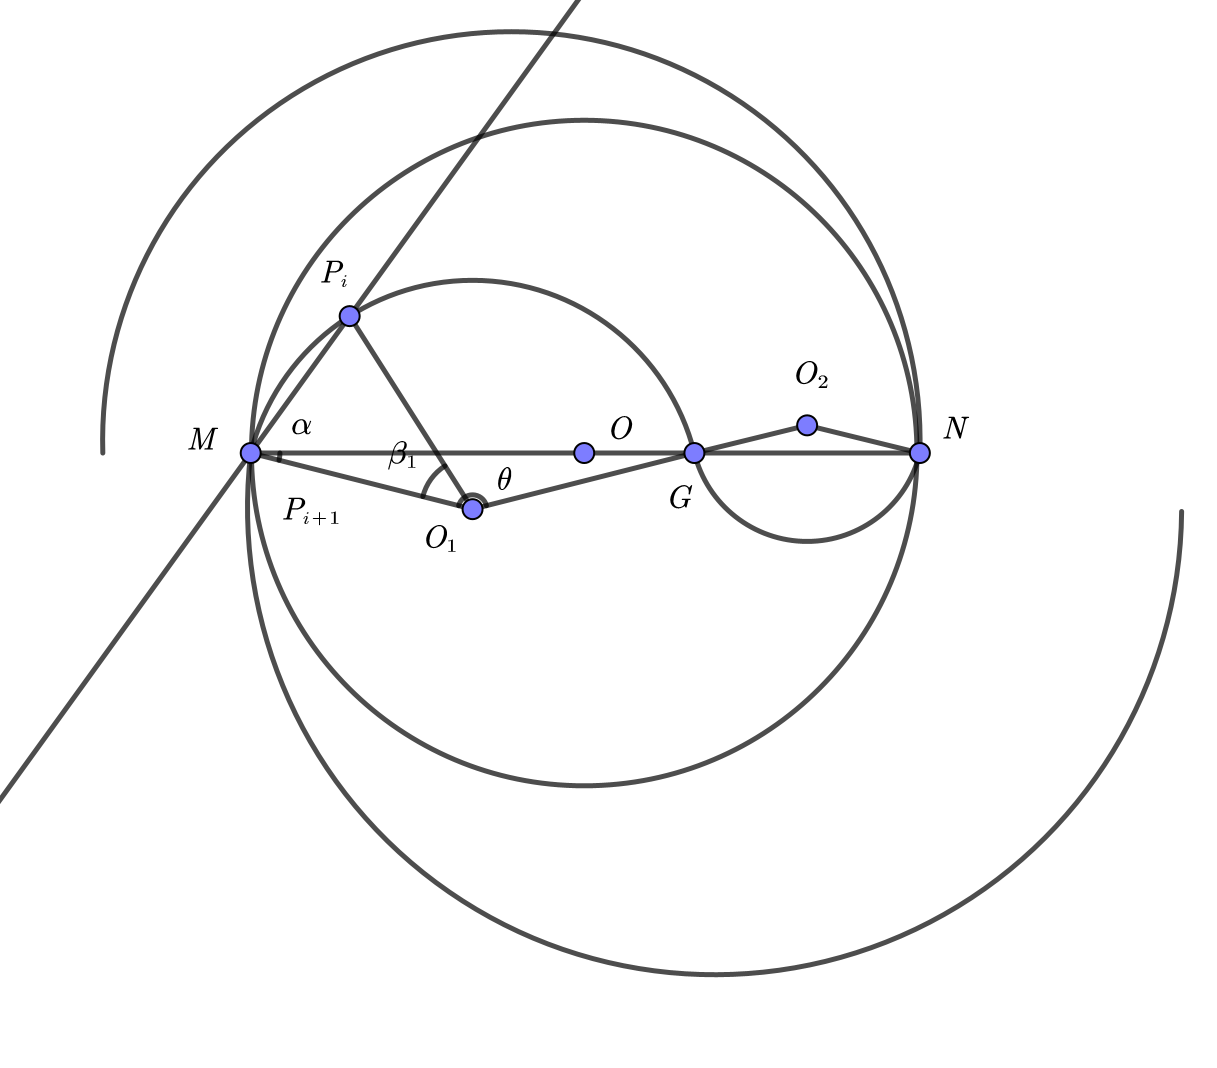
\includegraphics[width=.6\textwidth]{3}
\caption{几何示意图1}
\end{figure}
\par 在由点 \(P_{i}\)、\(O_{1}\) 和 \(P_{i + 1}\) 构成的三角形中,根据余弦定理有
\begin{align}
l_{i+1}^{2}=\left| \overrightarrow{P_iP_{i+1}} \right|^2=4r^2-4r^2\cos \beta _1.
\end{align}
由上式解得
\begin{align}\label{1.........443}
\beta _1=\left| \arccos \left( 1-\frac{l_{i+1}^{2}}{4r^2} \right) \right| = 
\end{align}
\begin{itemize}
\item \textbf{计算$\angle P_{i}(t)O_1M$}
\end{itemize}


根据几何关系及两直线夹角斜率公式可得
\begin{gather}\label{1.........444}
k_{O_1M}=\frac{y_M-y_{O_1}}{x_M-x_{O_1}},k_{O_1P_i\left( t \right)}=\frac{y_{P_i\left( t \right)}-y_{O_1}}{x_{P_i\left( t \right)}-x_{O_1}},
\\
\tan \angle P_i(t)O_1M=\frac{k_{O_1M}-k_{O_1P_i\left( t \right)}}{1+k_{O_1M}k_{O_1P_i\left( t \right)}}.
\end{gather}
\par 从而
\begin{align}\label{1.........445}
\angle P_i(t)O_1M= \arctan \frac{\frac{y_M-y_{O_1}}{x_M-x_{O_1}}-\frac{y_{P_i\left( t \right)}-y_{O_1}}{x_{P_i\left( t \right)}-x_{O_1}}}{1+\frac{y_M-y_{O_1}}{x_M-x_{O_1}}\cdot \frac{y_{P_i\left( t \right)}-y_{O_1}}{x_{P_i\left( t \right)}-x_{O_1}}}.
\end{align}
\begin{itemize}
\item \textbf{判断并计算$P_{i+1}$的位置}\label{subsubsection4.4.1.2}
\end{itemize}
    \par \(P_i\)在直线\(OM\)的上侧时,在得到\(\angle P_{i}(t)O_{1}M\) 和\(\beta_{1}\) 后,我们通过比较它们的大小来判断 \(P_{i + 1}\) 的位置.
    \par (1) 若$ \angle P_i(t)O_1M\in \left[ \beta _1,\theta \right]$ ,则\(P_{i + 1}\) 一定位于圆弧\(\wideparen{MG}\) 上.此时,我们可以根据以下两个方程来确定 \(P_{i + 1}\) 的坐标:
    \begin{align}\label{1.........446}
        \left\{ \begin{array}{c}
        \left( x_{i+1}-x_i \right) ^2+\left( y_{i+1}-y_i \right) ^2=l_{i+1}^{2}\\
        \left( x_{i+1}-x_{O_1} \right) ^2+\left( y_{i+1}-y_{O_1} \right) ^2=4r^2\\
        \end{array} \right. .
        \end{align}
\par 联立这两个方程求解,会得到\((x_{i + 1}, y_{i + 1})\) 的多个可能解。但结合题意可知,在这些解中,\(x_{i + 1}\) 的真实解是其中最小的一个,由此我们就能确定 \(P_{i + 1}\) 的直角坐标\((x_{i + 1}, y_{i + 1})\) .
\par (2)若$\angle P_i(t)O_1M< \beta_1$,则$P_{i+1}$一定位于盘入螺线$\varGamma$上.此时,我们利用问题1中建立的模型,按照相应的计算方法解出\((x_{i + 1}, y_{i + 1})\) 即可.
\par (3)若$\angle P_i(t)O_1M>\theta $,则进行下一步3  .

\textbf{
\begin{enumerate}[start=3]
    \item  判断$\angle P_{i}(t)O_2G$大小
 \end{enumerate}
}
\begin{itemize}
\item \textbf{引入判断角$\beta_2$}
\end{itemize}

\par 当第$t$秒$P_i(0\leq i\leq 222)$在$\wideparen{GN}$上时,引入判断角.若$P_{i+1}$与$G$点重合,则定义此时$\angle P_iO_2P_{i+1}=\beta_2$,称$\beta_2$为$\wideparen{GN}$判断角. 几何示意图如下:
\begin{figure}[H]
\centering
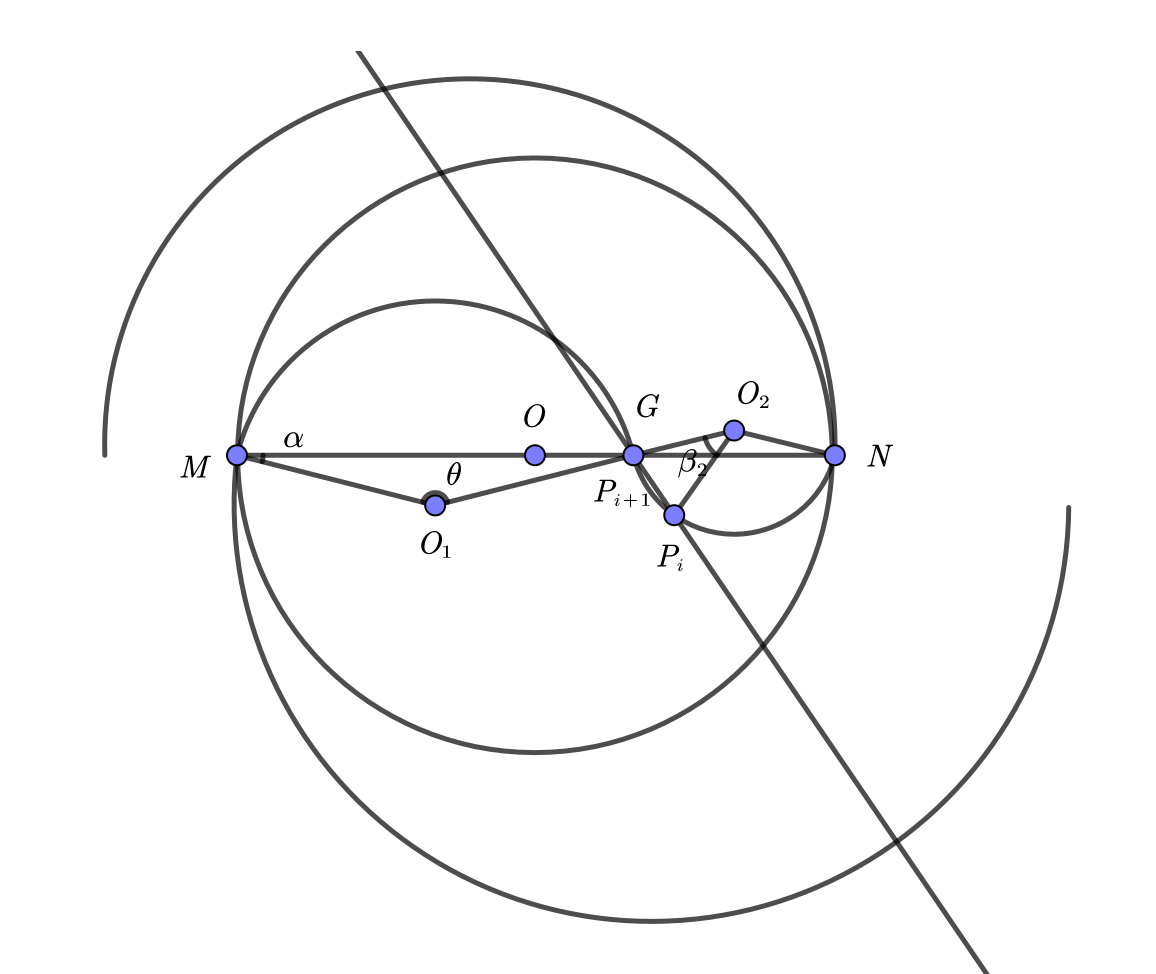
\includegraphics[width=.6\textwidth]{1}
\caption{几何示意图2}
\end{figure}
\par 在由点$ P_{i}$、$O_{2} $和 $P_{i + 1} $构成的三角形中,根据余弦定理有
\begin{align}\label{1.........448}
l_{i+1}^{2}=\left| \overrightarrow{P_iP_{i+1}} \right|^2=2r^2-2r^2\cos \beta _2.
\end{align}
由上式解得
\begin{align}\label{1.........449}
\beta _2=\left| \arccos \left( 1-\frac{l_{i+1}^{2}}{2R^2} \right) \right| = 
\end{align}

\begin{itemize}
\item \textbf{计算$\angle P_{i}(t)O_2G$}
\end{itemize}

\par 根据几何关系及两直线夹角斜率公式可得
\begin{gather}\label{1.........450}
k_{O_1O_2}=\frac{y_{O_2}-y_{O_1}}{x_{O_2}-x_{O_1}},k_{O_2P_i\left( t \right)}=\frac{y_{P_i\left( t \right)}-y_{O_2}}{x_{P_i\left( t \right)}-x_{O_2}},
\\
\tan \angle P_i(t)O_2G=\frac{k_{O_1O_2}-k_{O_2P_i\left( t \right)}}{1+k_{O_1O_2}k_{O_2P_i\left( t \right)}}.
\end{gather}
\par 从而
\begin{align}\label{1.........451}
\angle P_i(t)O_2G=\arctan \frac{\frac{y_{O_2}-y_{O_1}}{x_{O_2}-x_{O_1}}-\frac{y_{P_i\left( t \right)}-y_{O_2}}{x_{P_i\left( t \right)}-x_{O_2}}}{1+\frac{y_{O_2}-y_{O_1}}{x_{O_2}-x_{O_1}}\frac{y_{P_i\left( t \right)}-y_{O_2}}{x_{P_i\left( t \right)}-x_{O_2}}}.
\end{align}
\begin{itemize}
    \item \textbf{判断$\angle P_{i}(t)O_{2}G $并计算$P_{i+1}$的位置}
\end{itemize}
\par 在得到$\angle P_{i}(t)O_{2}G $和$\beta_{2} $后,通过比较它们的大小来判断 $P_{i + 1} $的位置。
 \par (1)若$\angle P_{i}(t)O_{2}G \in \left[ \beta _2,\theta \right]$ ,
根据几何关系可知,$P_{i + 1}$ 一定位于圆弧$\wideparen{GN} $上。此时,我们可以根据以下两个方程来确定 $P_{i + 1} $的坐标
\begin{align}\label{1.........452}
\left\{ \begin{array}{c}
\left( x_{i+1}-x_i \right) ^2+\left( y_{i+1}-y_i \right) ^2=l_{i+1}^{2}\\
\left( x_{i+1}-x_{O_2} \right) ^2+\left( y_{i+1}-y_{O_2} \right) ^2=r^2\\
\end{array} \right. .
\end{align}

\par 联立这两个方程求解,会得到$(x_{i + 1}, y_{i + 1}) $的多个可能解。由题意可知,$x_{i + 1} $的真实解是其中最小的一个。通过这种方式,我们确定了$P_{i + 1} $的直角坐标$(x_{i + 1}, y_{i + 1})$ 。
\par (2)若$\angle P_i(t)O_2G< \beta_2$,则$P_{i+1}$一定位于圆弧$\wideparen{MG}$上.从而根据2中的情形(1)解出$(x_{i+1},y_{i+1})$即可.
\par (3) 若$\angle P_i(t)O_2G>\theta$ ,则进行下一步 4 .
\textbf{
\begin{enumerate}[start=4]
    \item  判断$\angle P_{i}(t)O_2N$大小
 \end{enumerate}
}
\begin{itemize}
\item \textbf{引入判断角$\beta_3$}
\end{itemize}

\par 当第$t$秒$P_i(0\leq i\leq 222)$在$\varGamma'$上时,引入判断角.若$P_{i+1}$与$N$点重合,则定义此时$\angle P_iO_2N=\beta_3$,称$\beta_3$为$\varGamma'$判断角. 几何示意图如下:
\begin{figure}[H]
\centering
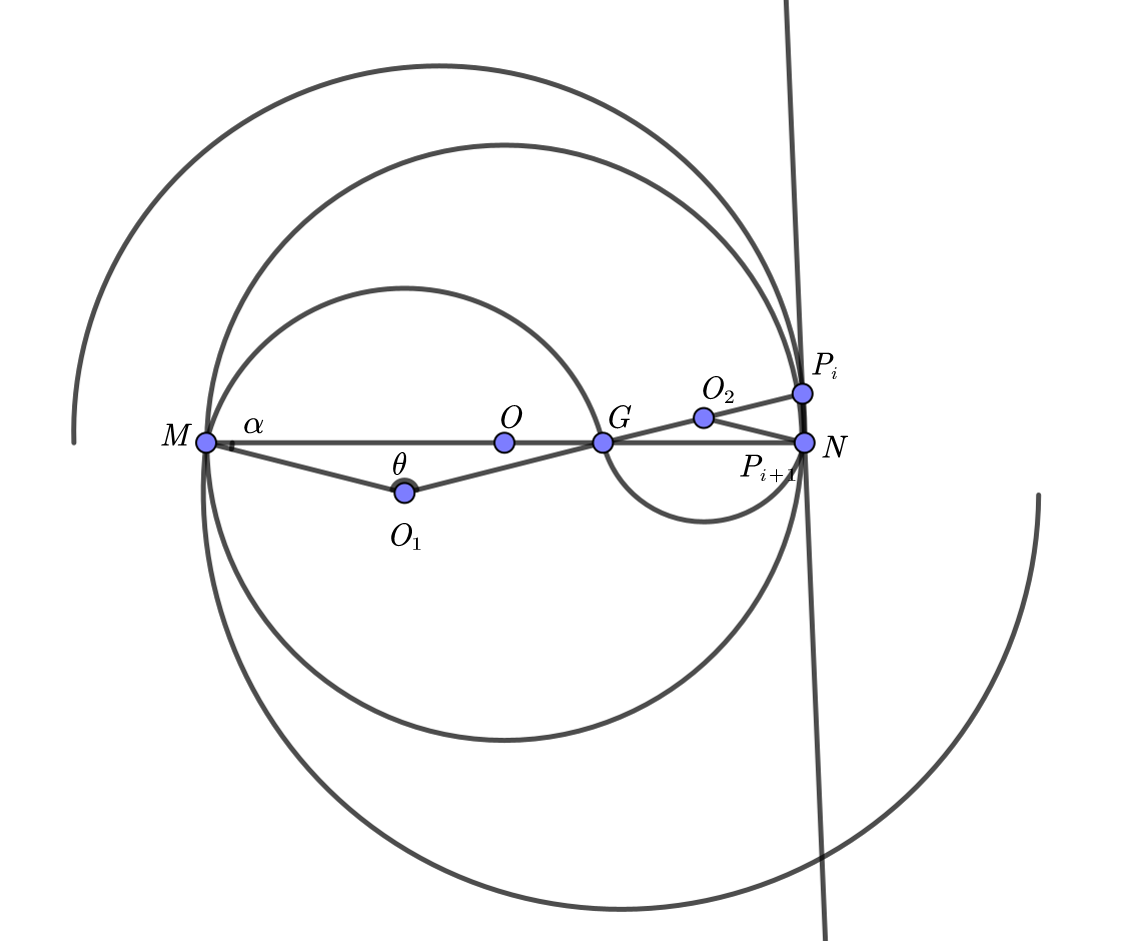
\includegraphics[width=.6\textwidth]{2}
\caption{几何示意图3}
\end{figure}
\par 在由点 \(P_{i}\)、\(O_{2}\) 和 \(P_{i + 1}\) 构成的三角形中,根据余弦定理有

\begin{gather}\label{1.........454}
\left| \overrightarrow{O_2P_i} \right|=\sqrt{\left( x_{P_i}-x_{O_2} \right) ^2+\left( y_{P_i}-y_{O_2} \right) ^2},
\\
l_{i+1}^{2}=\left| \overrightarrow{P_iP_{i+1}} \right|^2=\left| \overrightarrow{O_2P_i} \right|^2+r^2-2r\left| \overrightarrow{O_2P_i} \right|\cos \beta _3.
\end{gather}
由上式解得
\begin{align}\label{1.........455}
\beta _3=\left| \arccos \frac{r^2+\left( x_{P_i}-x_{O_2} \right) ^2+\left( y_{P_i}-y_{O_2} \right) ^2-l_{i+1}^{2}}{2r\sqrt{\left( x_{P_i}-x_{O_2} \right) ^2+\left( y_{P_i}-y_{O_2} \right) ^2}} \right| =
\end{align}

\begin{itemize}
\item \textbf{计算$\angle P_{i}(t)O_2N$}
\end{itemize}

\par 根据几何关系及两直线夹角斜率公式可得
\begin{gather}\label{1.........456}
k_{O_2N}=\frac{y_{O_2}-y_N}{x_{O_2}-x_N},k_{O_2P_i\left( t \right)}=\frac{y_{P_i\left( t \right)}-y_{O_2}}{x_{P_i\left( t \right)}-x_{O_2}},
\\
\tan \angle P_i(t)O_2N=\frac{k_{O_2N}-k_{O_2P_i\left( t \right)}}{1+k_{O_2N}k_{O_2P_i\left( t \right)}}.
\end{gather}
从而
\begin{align}\label{1.........457}
\angle P_i(t)O_2N=\arctan \frac{\frac{y_{O_2}-y_N}{x_{O_2}-x_N}-\frac{y_{P_i\left( t \right)}-y_{O_2}}{x_{P_i\left( t \right)}-x_{O_2}}}{1+\frac{y_{O_2}-y_N}{x_{O_2}-x_N}\frac{y_{P_i\left( t \right)}-y_{O_2}}{x_{P_i\left( t \right)}-x_{O_2}}} .
\end{align}
\begin{itemize}
    \item \textbf{判断并计算$P_{i+1}$的位置}
    \end{itemize}
    \par 在得到$\angle P_{i}(t)O_{2}N$和$\beta_{3}$后,通过比较它们的大小来判断 $P_{i + 1} $的位置。
 
    \par (1)若$\angle P_{i}(t)O_{2}N \geq \beta_{3}$,根据几何关系可知,$P_{i + 1}$一定位于盘出螺线$\Gamma'$上。此时,根据盘出螺线的性质以及两把手之间的距离关系,我们可以列出以下方程来确定$ P_{i + 1} $的坐标

\par 若$\angle P_{i}(t)O_{2}N \geq \beta_{3}$,根据几何关系可知,$P_{i + 1}$一定位于盘出螺线$\Gamma'$上。此时,根据盘出螺线的性质以及两把手之间的距离关系,我们可以列出以下方程来确定$ P_{i + 1} $的坐标

\begin{gather}\label{1.........458}
l_{i+1}^{2}=|P_i(t)P_{i+1}(t)|^2=(\rho _i(t))^2+(\rho _{i+1}(t))^2-2\rho _i(t)\rho _{i+1}(t)\cos\mathrm{(}\theta _i(t)-\theta _{i+1}(t)),
\\
\rho _{i+1}(t)=\frac{d_0}{2\pi}\left( \theta _{i+1}(t)+\pi \right) .
\end{gather}
\par 根据上式利用Python求解\(\theta _{i}(t)\),可能得到多个不同解.不妨设这些为不同的解为\(\alpha _{j}^{i}(t) (j = 1,2,\cdots ,m)\),注意到一定有\(\theta _{i}(t)<\theta _{i-1}(t)\),因此令
\begin{align}\label{1.........459}
A_i = \{ \alpha _{j}^{i}(t) |\alpha _{j}^{i}(t) <\theta _{i-1}(t),j = 1,2,\cdots ,m \},
\end{align}
\par 因为第\(i + 1\)个把手与第$i$个把手的极角之差一定是最小的,所以
\begin{align}\label{1.........460}
\theta _{i+1}(t)=\underset{\alpha _{j}^{i}(t)\in A_i}{\min}\left[ \alpha _{j}^{i}\left( t \right) -\theta _i\left( t \right) \right] +\theta _i\left( t \right) .
\end{align}
\par 将上述求得的\(\theta _{i+1}(t)\)代入盘入螺线$\varGamma'$得到此时\(P_{i+1}(t)\)的极坐标\((\rho _{i+1}(t),\theta _{i+1}(t))\).再利用极坐标与直角坐标之间的转化公式
\begin{align}\label{1.........461}
\begin{cases}
x_{i+1}(t)=\rho _{i+1}(t)\cos \theta _{i+1}(t)\\
y_{i+1}(t)=\rho _{i+1}(t)\sin \theta _{i+1}(t)\\
\end{cases}, 
\end{align}
\par 就能得到\(P_{i+1}(t)\)的直角坐标\((x_{i+1}(t),y_{i+1}(t))\).

\par (2)若$\angle P_i(t)O_2N< \beta_3$,则$P_{i+1}$一定位于圆弧$\wideparen{GN}$上.从而利用3的情形(1)解出$(x_{i+1},y_{i+1})$即可.

\par 综上,将$P_0$在不同时刻的坐标代入上述四个步骤,不断递推就能得到所有把手的位置坐标.
\\\noindent\textbf{Step 7 计算板凳龙从-100s到100s各把手的速度} 
\par 由Step 5,Step 6,我们可以得到板凳龙各把手不同时刻在极坐标系下的的位置坐标,因此利用问题一中求得的速度迭代公式
\begin{small}
\begin{align}
v_i(t) = \sqrt{\frac{1 + {\theta _i}^2}{1 + {\theta _{i - 1}}^2}}\frac{|-\theta _{i - 1}+\theta _i\cos(\theta _{i }-\theta _{i-1})+\theta _i\theta _{i - 1}\sin(\theta _{i }-\theta _{i-1})|}{|\theta _i+\theta _i\theta _{i - 1}\sin(\theta _i -\theta _{i-1})-\theta _{i - 1}\cos(\theta _i -\theta _{i-1})|} v_{i - 1}(t), i\in \{1, 2, \cdots, 223\},
\end{align}
\end{small}
\par  因此,令\(i\)依次取\(1, 2, \cdots, 223\),利用Python进行迭代计算,就能得到板凳龙的第\(i(1\leqslant i\leqslant 223)\)节板凳的后把手中心在第\(t\)秒时的速度\(v_i(t)\).
再令\(t\)依次取$(-100, -99, \cdots, 100)$,反复进行上述操作,就能得到板凳龙板凳龙从-100s到100s各把手的速度.  

\end{document}